

\chapter{Background}\label{chapter:background}


\section{Large Language Model}


Large Language Models (LLMs) are highly complex artificial intelligence systems that can learn from the vast amounts of available text data\cite{radford2018improving}. Thanks to the attending of \textit{Transformer}\cite{vaswani2017attention}, a deep learning architecture, these language models which employed self-supervised pre-training have demonstrated improved efficiency and scalability in many fields.

Based on self-attention mechanisms and feed-forward module, \textit{Transformer} has overwhelming advantages in computing representations and global dependencies.

In concrete terms, the Large Language Models equipped with \textit{Transformer} are capable of diverse tasks raised by Natural Language Processing\cite{chowdhary2020natural}, such as textual entailment, question answering, semantic similarity assessment, and document classification. Take BERT\cite{alaparthi2020bidirectional} and GPT\cite{radford2018improving,radford2019language,brown2020language} as two examples, the former utilizes transformer encoder blocks to predict missing words in a given text, and the latter has been enjoying a tremendous reputation for generating diverse and human-like responses, showcasing its potential in various domains.

    \subsection{Text Classification}
In our project, a bunch of hierarchical activity labels would be acquired from the dataset \textit{drive \& act} to depict every detail of the participant's movements in the driving behavior recorded in the video. These labels, however, are too trivial for the construction of learning data, as considering each activity individually will be tedious in such a vast and complex model training process. Therefore, labels should be classified according to the object on which this behavior operates or the specificity of the moment in which the action takes place. For example, the fastening of a seat belt should occur shortly after entering the vehicle, and all behavior related to eating or drinking should be classified into the same group.

In our task, we use zero-shot text classification. This is a task where a model is trained on a set of labeled examples and then classifies new examples from previously unseen classes. This method, which leverages a pre-trained language model, can be thought of as an instance of transfer learning which generally refers to using a model trained for one task in a different application than what it was originally trained for. This is particularly useful for situations where the amount of labeled data is small, for example, our work with 39 different behaviors to be classified.

The model used in the pipeline is \textit{BART} \cite{lewis2019bartdenoisingsequencetosequencepretraining}. According to the paper, BART is trained by corrupting text with an arbitrary noising function and learning a model to reconstruct the original text. It uses a standard Tranformer-based neural machine translation architecture, which, despite its simplicity, can be seen as generalizing BERT (due to the bidirectional encoder), GPT (with the left-to-right decoder), and many other more recent pre-training schemes. With all these prerequisites, it is quite obvious that \textit{BART} is a very practical model for our classification task.



\section{Hidden Markov Model}
Hidden Markov Model(HMM) \cite{rabiner1989tutorial,baum1972inequality} is one of the earliest probabilistic models for sequential data analysis.It is a Markov model in which the observations are dependent on a latent (or hidden) Markov process. A detailed introduction could be found in~\ref{chapter:appendix}. HMM do have wide applications in fields such as early speech recognition, part-of-speech tagging, and bioinformatics, where sequences of discrete states and short-term dependencies were dominant. However, limits such as assuming a fixed number of discrete states and being limited by the first-order Markov property (current state only depends on the previous state) could draw back the results when too much feature information is involved. In this work we use HMM as the baseline of our model in order to compare the performance of our model with the traditional one.
\section{Graph}
\label{sec:graph}
In graph theory, a graph is a structure made up of a collection of objects, where certain pairs of these objects are connected in a specific way\cite{zhou2020graph}. As a powerful tool for modeling and analyzing complex systems, researchers have combined graph theory with deep learning to solve various problems in different fields, such as social networks\cite{wu2020graph}, complex physic system\cite{sanchez2018graph} and Protein-protein interactions (PPIs)\cite{NIPS2017_f5077839}.

A Graph is $\mathcal{G} = (\mathcal{V}, \mathcal{E})$ is a pair of sets, where collections of \textit{nodes} $\mathcal{V}$ and edges $\mathcal{E} \subseteq \mathcal{V}\times \mathcal{V}$ between pairs of nodes. The nodes here are assumed as the nodes to be endowed with s-dimensional \textit{node feature}, denoted by $x_u$ for all $u\in \mathcal{V}$. Taking social network as an example, nodes represent users, and edges correspond to the friendship relations between them. The features of nodes model user properties such as age, likelihood, etc. Also, some models, including this work, would endow the edges with features. In generic setting $\mathcal{E} \neq 0$, the node features are rows of the $x\times d$ matrix $X=(x_1,\ldots,x_n)^T$. To apply some function to update the features in every node, obtaining the set of latent node feature, we would introduce permutation equivariant function $H=F(X)$, where $H$ is the feature matrix whose $u$th row is the latent feature of node $u$.

As for the edges $e\in \mathcal{E}$, or the graph connectivity, they can be represented by the $n\times n$ adjacency matrix $A$ defined as 
\[a_{uv} = \left\{ \begin{array}{rcl}
1 & (u,v)\in \mathcal{E} \\ 0 & otherwise 
\end{array}\right.\]

Here $a_{uv}$  specifies the adjacency information between the nodes described by the $u$th and the $v$th rows of $X$.
Most functions acting on graphs can be viewed as the generators for 'local' node-wise output, i.e., whereby the output on node $u$ directly depends on its neighboring nodes in the graph. It is worthwhile formalizing this constraint explicitly in our model construction by defining what it means for a node to be neighboring another. An (undirected) neighborhood of node $u$ is defined as 
\[\mathcal{N}_u = \{v : (u,v) \in \mathcal{E} \text{ or } (v,u) \in \mathcal{E}\}\]
and the neighborhood features as the multiset\cite{10.48550/arxiv.2104.13478}.
\[\mathcal{X}_{\mathcal{N}_u}={{x_v:v\in N}}\]

Thus, the features of a node as well as its neighborhood could be collected simultaneously by a local function $\phi(x_u,\mathcal{X}_{\mathcal{N}_u}) $. Then the permutation equivariant function $F$ can be constructed by applying $\phi$ to every node's neighborhood in isolation (Figure~\ref{fig:graphupdate}).

$$ F(X,A) = \left[ \begin{array}{rcl}
-- & \phi(x_1,\mathcal{X}_{\mathcal{N}_1}) & -- \\
-- & \phi(x_2,\mathcal{X}_{\mathcal{N}_2}) & -- \\
& \vdots & \\
-- & \phi(x_n,\mathcal{X}_{\mathcal{N}_n}) & --\\

    
\end{array}\right] $$

\begin{figure}[h]
    \centering
    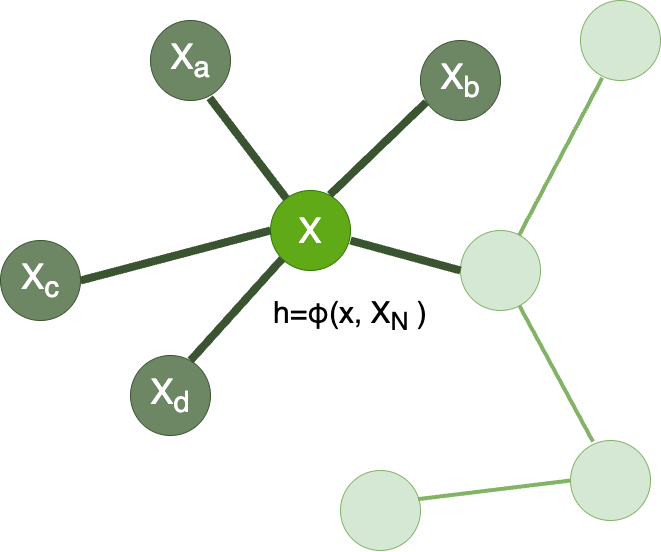
\includegraphics[width=0.5\textwidth]{figures/02_GraphFeature.png}
    \caption{Constructing permutation equivariant functions over graphs.}
    \label{fig:graphupdate}
\end{figure}



    \subsection{Graph Neural Networks}
    The intuitive understanding among \textbf{Graph Neural Network (GNN)} is that nodes in a graph represent objects or concepts, and edges represent their relationships. Each concept is naturally defined by its features and the related concepts\cite{10.1109/tnn.2008.2005605}. GNNs are among the most general class of deep learning architectures currently in existence, and most learning architectures can be understood as a special case of the GNN with additional geometric structure. 
    
    Given to the mathematic expression we have settled in section~\ref{sec:graph} we consider a graph to be specified with an adjacency matrix $A$ and node feature $X$. The GNN architectures we study arepermutation equivariant functions $F(X,A)$  construcetd by applying shared permutation invariant function $\phi(x_u,\mathcal{X}_{\mathcal{N}_u}) $ over local neighborhood. This function $\psi$ would be referred to as "diffusion", "propagation", or "message passing", and the all over computation of such of such $F$ as a "GNN layer".

    The design and study of GNN layers is one of the most active area of deep learning in the recent past few years. And three vast "flavours" of GNN layers are derived from the vast majority of the literatures. These flavours govern the extent to which $\psi$ transforms the neighbourhood features, allowing for varying degrees of complexity when modelling interactions across the graph(Figure~\ref{fig:graphlayer}). 
    
    \begin{figure}[h]
        \centering
        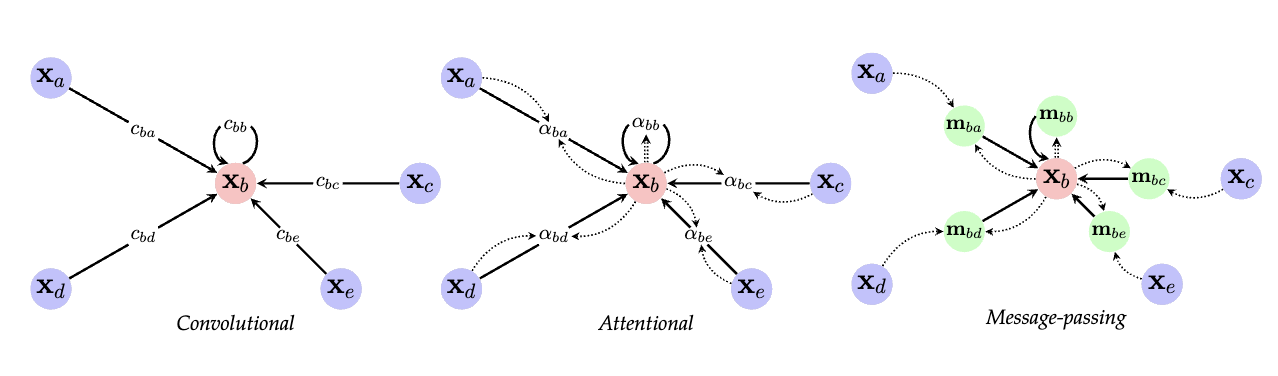
\includegraphics[width=\textwidth]{figures/02_GNNlayers.png}
        \caption{A visualisation of the dataflow for the three flavours of GNNlayers. Reproduced from \cite{10.48550/arxiv.2104.13478}}
        \label{fig:graphlayer}
    \end{figure}

    In all the three flavours, the feature update function for node $u$ would apply permutation-invariant function $\oplus$ to aggregate features from $\mathcal{X}_{\mathcal{N}_u}$ ,as well as learnable function $\psi$. The function $\oplus$ is potentially transformed, by means of some function $\psi$ and itself is usually realized as a nonparametric operation such as sum, mean, or maximum.


    In the \textbf{convolution flavour}\cite{kipf2016semi,defferrard2016convolutional,wu2019simplifying}The feature of the neighborhood nodes are directly aggregated with fixed weights $c_{uv}$, which often directly depends on the entries in $A$ representingthe structure of the graph. The update function is defined as:
    \[
    \mathbf{h}_u = \phi \left( \mathbf{x}_u, \bigoplus_{v \in \mathcal{N}_u} c_{uv} \psi(\mathbf{x}_v) \right).
    \]


    In the \textbf{attention flavour}\cite{velickovic2017graph,monti2017geometric,zhang2018gaan}the weights $c_{uv}$ are replaced by the a learnable self-attention mechanism that computes the importancecoefficients. And the update function is defined as:

    \[
        \mathbf{h}_u = \phi \left( \mathbf{x}_u, \bigoplus_{v \in \mathcal{N}_u} a(x_u,x_v) \psi(\mathbf{x}_v) \right).
    \]

    And the \textbf{message-passing flavour}\cite{gilmer2017neural,battaglia2018relational} aims at computing arbitrary vectors of neighborhood $\mathcal{N}_u$ send to $u$, where vector-based messages are computed based on both the sender and receiver: $m_{uv} = \psi (x_u, x_v)$.
    \[
        \mathbf{h}_u = \phi \left( \mathbf{x}_u, \bigoplus_{v \in \mathcal{N}_u} \psi (x_u, x_v) \right).
    \]

    What matters is that a representational containment between these approaches exists: $convolution \in attention \in message-passing $. This, however, does not mean that message-passing is always the most useful choice. Indeed, the vector-based messages always contains most oriented information across the edges, but they are harder to train due to the enormous requirement of memories. And here, in our work, we have such a specific network that none of the approaches above is the best choice.
 

    \subsection{Dynamic graph}
    Our discussion so far has focused solely on input that exhibits spatial variations across a given domain; however, the input may also change over time, for instance, video, text or speech.
    Assume that the input consists of arbitrary steps, and an input signal will be provided at each step $t$, we represent as $X^{(t)}\in \mathcal{X} (\omega^{(t)})$.

    While in many cases the domain in kept fixed across time $t$, we notice that exceptions also happens. For example in our work, we many find tremendous changes in the videos from our dataset. Such domain as changing over time is referred to as \textit{dynamic graph}\cite{rossi2006temporal,xu2020inductive}.

    Assume an encoder function $f(X^(t))$ offering latent presentation for such dynamic graph learning problem. In the video analysis, $\omega$ is a fixed grid, and signals are a sequence of frames. To have a view of the entire frame, one of the options is to implement $f$ as a translation invariant CNN, outputting a k-dimensional representation $z(t)=f(X^(t))$  of the frame at time-step $t$. In our work, however, we use an alternative approaches, which we would introduce in chapter\ref{chapter:relatedwork}.

    To have a canonical analysis for dynamically aggregate the sequence of vectors $z(t)$, we introduce \textit{Recurrent Neural Network} (RNN)\cite{schmidt2019recurrent} due its advantages in the field of temporal progression of inputs and online arrival of novel data-points. A clear view of analyzing video data with RNN is given in Figure~\ref{fig:RNN}.

    \begin{figure}[h]
        \centering
        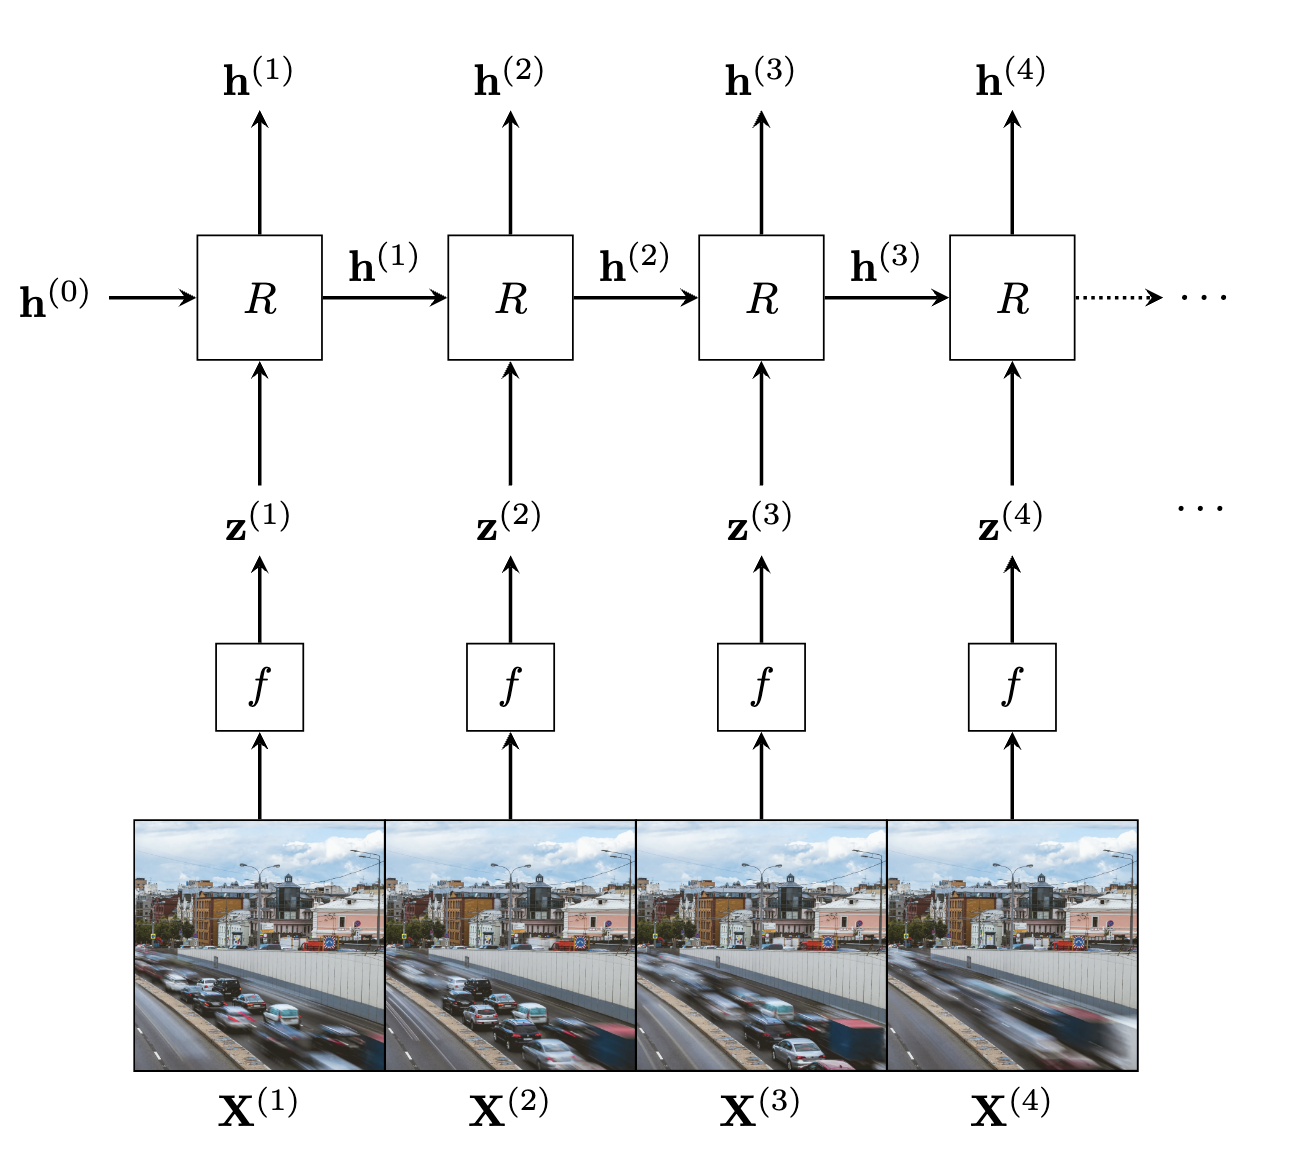
\includegraphics[width=0.7\textwidth]{figures/02_RNN.png}
        \caption{Illustration of processing video input with RNNs. Reproduced from \cite{10.48550/arxiv.2104.13478}}
        \label{fig:RNN}
    \end{figure}

    A simple RNN model is defined as the following way: The model holds with an m-dimensional summary vector $h(t)$ of all the input steps up to and including $t$. This will summarize the current step's features as well as the information collected from the past, through a shared function $R: \mathbb{R} ^k \times \mathbb{R} ^m \rightarrow \mathbb{R} ^m$, as follows:
    \[
        h(t) = R(z(t), h(t-1))
    \]

    As both $z(t)$ and $h(t-1)$ are vectors, the function $R$ is usually realized as a simple feed-forward neural network(often known as \textit{Simple RNN}\cite{elman1990finding,jordan1997serial}):
    \[
        h(t) = \sigma(W_z z(t) + U h(t-1) + b)
    \]
    Where $W_z$ and $U$ are the weight matrices, $b$ is the bias, and $\sigma$ is the activation function. 

    The summary vectors may then be appropriately leveraged for the down-stream task—if a prediction is required at every step of the sequence, then a shared predictor may be applied to each $h(t)$ individually. For classifying entire sequences, typically the final summary, $h(T)$, is passed to a classifier, just like many works including ours.


    

\section{behavior prediction for human driver}

The earliest research regarding the prediction of human driver behavior could be dated back to the 1990s, when hidden Markov models are first introduced to model the driver's behavior\cite{10.1162/089976699300016890}. An HMM is a statistical model that represents a system with hidden states, where observable outputs are generated by these underlying, unobservable states. Each state transitions to another with a certain probability and emits observations based on specific probability distributions. 

The paper is constructed on the ground truth that the intended actions, like to turn or change lanes, are modeled as a sequence of internal states. By observing the temporal patterns of the driver's behavior or even intention. Although the attempt then is to capture and predict driver eye movements in the context of lane keeping/curve negotiation and car following to determine. It still proves that characteristic patterns in driver behavior could be identified and even represent by mathematical models.

With the advancement of various machine learning models, more sophisticated tools have emerged, expanding the range of options available for predicting human driver behavior. In \cite{10.1109/ivs.2018.8500717}, hidden Markov models are adapted for this topic as well, yielding promising results due to the enhanced computational capabilities available today. Another study \cite{10.1109/icra40945.2020.9196918} proposes an LSTM-based trajectory prediction method for human drivers, which facilitates better decision-making for autonomous vehicles, particularly in urban intersection scenarios. Despite these significant achievements, there remains a noticeable gap in driver behavior prediction for driver-oriented dynamic scene graphs. Such an approach could capture individual driving habits, enabling more precise predictions and even anomaly detection tailored to each driver. Our work aims to address this gap.